\chapter{Conceitos Básicos}
\label{sec:conceitos}

\section{Servidores e listas de servidores em jogos eletrônicos}
\label{sec:conceitos:servidores}
    TODO

\section{Redes Distribuídas}
\label{sec:conceitos:redes}
    TODO

\section{Vikings}
\label{sec:conceitos:vikings}
  O \textit{vikings}\footnotemark{} é um software livre produzido numa experiência de mini-projetos realizada pelo USPGameDev\footnotemark. 
  Foi desenvolvido em Janeiro e Fevereiro de 2013 por Henrique Gemignani Passos Lima e Wilson Kazuo Mizutani 
  utilizando a LÖVE, um arcabouço para jogos 2D em Lua\footnotemark{}.
  
  \begin{figure}
    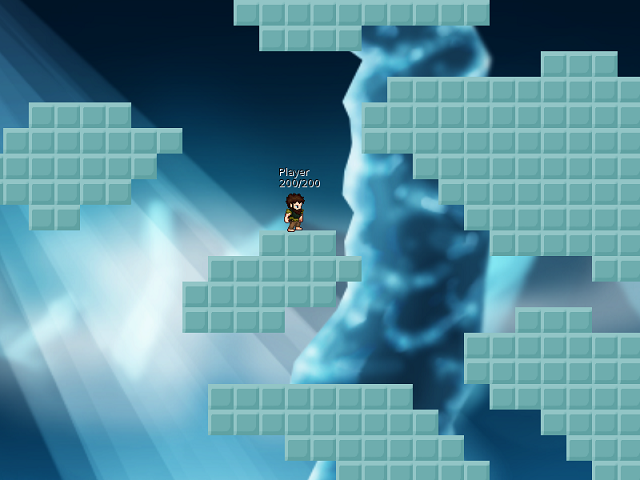
\includegraphics{imagens/vikings-1.png}
    \caption{Imagem do vikings}
  \end{figure}
  
  \addtocounter{footnote}{-3}

  \stepcounter{footnote}\footnotetext{
    Página do projeto: \url{http://uspgamedev.org/projetos/vikings/} (última visita em 23/11/2013).
  }
  \stepcounter{footnote}\footnotetext{
    O USPGameDev é um grupo de pesquisa e desenvolvimento de jogos da
    Universidade de São Paulo. Ver \url{http://uspgamedev.org/} (última visita em 03/09/2013).
  }
  \stepcounter{footnote}\footnotetext{
    Página oficial: \url{http://www.lua.org/} (última visita em 23/11/2013).
  }

  \subsection{O Jogo}
    Em \textit{vikings}, você controla um jovem viking que sonha em se tornar o líder de sua vila. Para tal,
    você sai em busca de aventuras, buscando experiência, riquezas e equipamentos poderosos, para que um dia,
    você seja forte o suficiente para desafiar e derrotar o seu líder, tomando o seu lugar.
        
  \subsection{Jogabilidade}
    É um jogo de plataforma 2D com gráficos 2D, com mapas gerados proceduralmente. Com o intuito de garantir
    que todo mapa gerado é possível, e numa tentativa de introduzir alguma profundidade e dificuldade, é
    possível dar quantas \textit{arrancadas} você quiser, mesmo estando no ar, e um único pulo no ar. No
    entanto, bater com a sua arma numa parede concede mais um pulo, permitindo ao jogador que ele escale
    paredes.
    
  \subsection{Detalhes Técnicos}
    Uma lista de conceitos e/ou algorítimos interessantes presentes no código:
    
    \subsubsection{Orientação a Objetos}
      Lua não possui orientação a objetos nativamente, mas utilizando as ferramentas da linguagem é possível
      implementar um sistema de orientação a objetos baseada em protótipos.
      No projeto, utilizamos o LUX\footnotemark{}, escrito pelo próprio Wilson, em vez de repetir uma implementação.
      
      \footnotetext{
        Página do projeto: \url{https://github.com/Kazuo256/luxproject} (última visita em 23/11/2013).
      }
    
    \subsubsection{Geração procedural de conteúdo}
      Para a geração dos mapas de cavernas, utilizamos o algorítimo de automato celular, descrito no RogueBasin,
      \cite{roguebasin:cellularautomata} e levemente alterado para criar plataformas mais largas. Para
      evitar problemas de áreas desconexas, há um tratamento posterior do mapa onde áreas desconexas são unidas.
      Por fim, procuramos por plataformas vazias onde popular com monstros e itens.